%%=============================================================================
%% Resultaten
%%=============================================================================

\chapter{Resultaten}
\label{ch:resultaten}

Om de verschillende modellen te testen, worden meerdere scenario’s gehanteerd.
Ten eerste wordt gebruikgemaakt van een testset met tien vragen waarvan de informatie beschikbaar is in de documentatie. Van elk model wordt verwacht dat het op iedere vraag een concreet antwoord geeft. Deze antwoorden worden vervolgens geëvalueerd met behulp van het test framework Ragas, waarbij vier verschillende meetcriteria worden toegepast.
\\[1em]
Het tweede testscenario bestaat uit het stellen van niet-triviale vragen waarvoor de informatie niet beschikbaar is in de documentatie. Dit scenario is vooral bedoeld om te onderzoeken of bepaalde modellen tekenen van hallucinaties vertonen.
\\[1em]
Als laatste worden enkele triviale vragen gesteld. Hierbij wordt getest of het model in staat is een juiste inschatting te maken door direct te antwoorden, zonder onnodige zoekopdrachten in de vector database.

\section{Evaluatie 1: Documentatiegebaseerde vragen}

Voor elk model werd een afzonderlijke vragenlijst opgesteld, waarbij de verwachte antwoorden zijn opgenomen in bijlage \ref{vragenlijst}.
De antwoorden die door de modellen zijn gegenereerd, zijn weergegeven in bijlage \ref{antwoordenlijst}.
In beide bijlagen zijn, uit overwegingen van gegevensbescherming, alle contactgegevens geanonimiseerd.
\\[1em]
Voor deze evaluatie wordt gebruikgemaakt van een testframework \textit{Ragas}. Tijdens de testen wordt voor iedere vraag de volgende informatie verzameld: de gebruikersinput, de opgehaalde context, het antwoord van de LLM en het verwachte antwoord. Op basis van deze gegevens gebruikt Ragas zelf een LLM om de dataset te beoordelen volgens de gekozen evaluatie criteria. In dit geval werd hiervoor het testmodel \texttt{gemma3:4b} gebruikt, omdat dit model een goede balans biedt tussen rekensnelheid, geheugengebruik en beoordelingskwaliteit. Hierdoor kon de evaluatie efficiënt worden uitgevoerd. Dit resulteert in een rapport waarin iedere vraag wordt beoordeeld op de verschillende criteria.
\\[1em]
De scores per vraag variëren tussen 0 en 1, waarbij een score van 1 een volledig correct antwoord representeert.
Binnen de categorie \textit{Faithfulness} geeft een score van 0{,}000 aan dat het model ten onrechte heeft nagelaten de retriever-tool te gebruiken, waardoor de opgehaalde context leeg bleef.
Voor de categorie \textit{Context Recall} kan dit in sommige gevallen juist het tegenovergestelde effect hebben: wanneer de opgehaalde context leeg is, kan het antwoord van het model toch een score van 1 behalen, mits het volledig aansluit bij de afwezigheid van context.
\\[1em]
De meetcriteria \textit{Faithfulness} beoordeelt hoe consistent het antwoord is met de opgehaalde context. \textit{Response relevancy} kijkt naar hoe relevant het antwoord is ten opzichte van de vraag. Onvolledige of overbodige informatie leidt hierbij tot een lagere score. \textit{Answer correctness} beoordeelt hoe correct het antwoord is in vergelijking met het verwachte antwoord, waarbij zowel feitelijke als semantische overeenkomsten worden meegenomen. \textit{Context recall} controleert in welke mate de benodigde informatie voor het antwoord aanwezig is in de opgehaalde context. Hoe groter de overlap tussen het juiste antwoord en de context, hoe hoger de score. Deze meetcriteria kijkt dus vooral naar hoe goed het model het ophaalproces aanstuurt.
\\[1em]
Op basis van deze evaluatie zijn de volgende resultaten vastgesteld:
\subsection{Llama3.1}

\begin{table}[H]
    \begin{tabular}{|l|c|c|c|c|}
        \hline
        \textbf{Vraag} & \textbf{Faithfulness} & \textbf{Response relevancy} & \textbf{Answer correctness} & \textbf{Context recall} \\
        \hline
        Vraag 1 & 1.000 & 0.000 & 0.225 & 0.500 \\
        Vraag 2 & 0.333 & 0.000 & 0.221 & 0.000 \\
        Vraag 3 & 0.385 & 0.000 & 0.223 & 0.500 \\
        Vraag 4 & 0.000 & 0.000 & 0.174 & 1.000 \\
        Vraag 5 & 1.000 & 0.863 & 0.212 & 0.125 \\
        Vraag 6 & 0.667 & 0.920 & 0.477 & 1.000 \\
        Vraag 7 & 0.500 & 0.000 & 0.205 & 1.000 \\
        Vraag 8 & 0.714 & 0.000 & 0.408 & 1.000 \\
        Vraag 9 & 0.500 & 0.932 & 0.391 & 1.000 \\
        Vraag 10 & 0.333 & 0.000 & 0.205 & 1.000 \\
        \hline
    \end{tabular}
    \caption{Resultaten per vraag op de vier meetcriteria van het Llama3.1 model.}
    \label{tab:resultaten_vragen_llama3.1}
\end{table}

\subsection{Llama3.2}

\begin{table}[H]
    \centering
    \begin{tabular}{|l|c|c|c|c|}
        \hline
        \textbf{Vraag} & \textbf{Faithfulness} & \textbf{Response relevancy} & \textbf{Answer correctness} & \textbf{Context recall} \\
        \hline
        Vraag 1  & 0.500 & 0.894 & 0.485 & 0.500 \\
        Vraag 2  & 0.333 & 0.000 & 0.220 & 0.000 \\
        Vraag 3  & 0.800 & 0.000 & 0.219 & 0.500 \\
        Vraag 4  & 0.571 & 0.863 & 0.196 & 0.833 \\
        Vraag 5  & 0.625 & 0.000 & 0.205 & 0.125 \\
        Vraag 6  & 0.857 & 0.000 & 0.194 & 1.000 \\
        Vraag 7  & 0.917 & 0.860 & 0.991 & 1.000 \\
        Vraag 8  & 0.833 & 0.953 & 0.212 & 1.000 \\
        Vraag 9  & 0.429 & 0.883 & 0.631 & 0.375 \\
        Vraag 10 & 0.333 & 0.000 & 0.207 & 1.000 \\
        \hline
    \end{tabular}
    \caption{Resultaten per vraag op de vier meetcriteria van het Llama3.2 model.}
    \label{tab:resultaten_vragen_llama3.2}
\end{table}

\subsection{Qwen2.5}

\begin{table}[H]
    \begin{tabular}{|l|c|c|c|c|}
        \hline
        \textbf{Vraag} & \textbf{Faithfulness} & \textbf{Response relevancy} & \textbf{Answer correctness} & \textbf{Context recall} \\
        \hline
        Vraag 1  & 0.750 & 0.000 & 0.485 & 0.500 \\
        Vraag 2  & 0.500 & 0.000 & 0.226 & 0.000 \\
        Vraag 3  & 0.929 & 0.000 & 0.229 & 0.500 \\
        Vraag 4  & 0.000 & 0.000 & 0.174 & 1.000 \\
        Vraag 5  & 0.000 & 0.000 & 0.180 & 0.000 \\
        Vraag 6  & 1.000 & 0.871 & 0.469 & 1.000 \\
        Vraag 7  & 0.000 & 0.000 & 0.176 & 1.000 \\
        Vraag 8  & 0.000 & 0.000 & 0.179 & 0.000 \\
        Vraag 9  & 0.000 & 0.000 & 0.176 & 0.556 \\
        Vraag 10 & 0.667 & 0.000 & 0.216 & 0.000 \\
        \hline
    \end{tabular}
    \caption{Resultaten per vraag op de vier meetcriteria van het Qwen2.5 model.}
    \label{tab:resultaten_vragen_qwen2.5}
\end{table}


\subsection{Qwen3}

\begin{table}[H]
    \begin{tabular}{|l|c|c|c|c|}
        \hline
        \textbf{Vraag} & \textbf{Faithfulness} & \textbf{Response relevancy} & \textbf{Answer correctness} & \textbf{Context recall} \\
        \hline
        Vraag 1  & 1.000 & 0.000 & 0.216 & 0.500 \\
        Vraag 2  & 1.000 & 0.000 & 0.224 & 0.000 \\
        Vraag 3  & 1.000 & 0.000 & 0.220 & 0.250 \\
        Vraag 4  & 0.857 & 0.000 & 0.203 & 0.000 \\
        Vraag 5  & 0.636 & 0.867 & 0.211 & 0.125 \\
        Vraag 6  & 0.750 & 0.874 & 0.571 & 1.000 \\
        Vraag 7  & 1.000 & 0.906 & 0.989 & 1.000 \\
        Vraag 8  & 0.556 & 0.000 & 0.411 & 1.000 \\
        Vraag 9  & 1.000 & 0.000 & 0.340 & 0.625 \\
        Vraag 10 & 1.000 & 0.935 & 0.636 & 1.000 \\
        \hline
    \end{tabular}
    \caption{Resultaten per vraag op de vier meetcriteria van het Qwen3 model.}
    \label{tab:resultaten_vragen_qwen3}
\end{table}


\subsection{Samenvatting}

Om de prestaties van de modellen per individuele metric te vergelijken, worden in figuur~\ref{fig:vergelijking_metrics} vier staafdiagrammen weergegeven: Faithfulness, Response relevancy, Answer correctness en Context recall.

\begin{figure}[H]
    \centering
    \begin{subfigure}{0.48\textwidth}
        \centering
        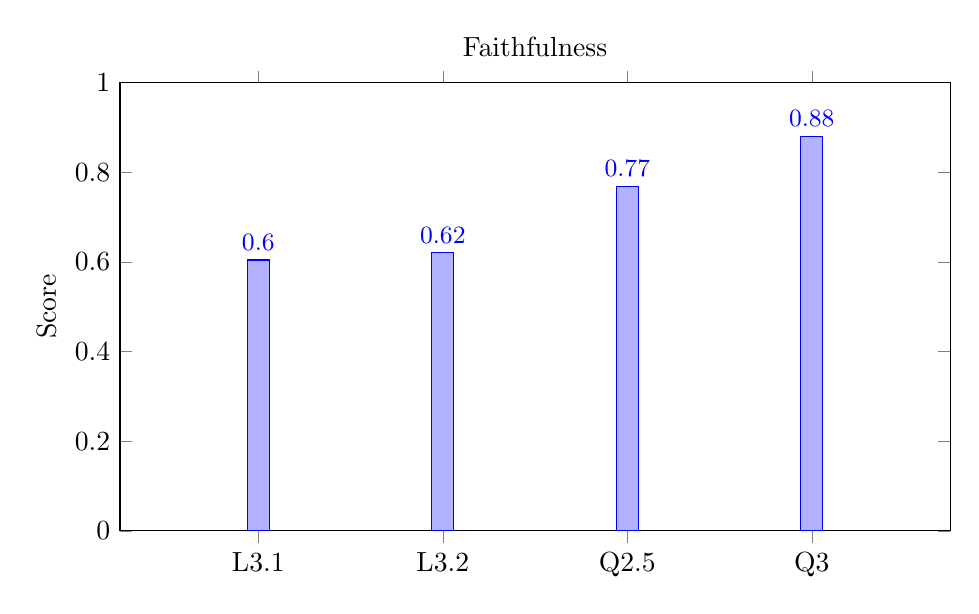
\begin{tikzpicture}
            \begin{axis}[
                ybar,
                ymin=0,
                ymax=1,
                bar width=8pt,
                width=\textwidth,
                height=0.6\textwidth,
                enlarge x limits=0.25,
                ylabel={Score},
                symbolic x coords={L3.1,L3.2,Q2.5,Q3},
                xtick=data,
                nodes near coords,
                nodes near coords align={vertical},
                every node near coord/.append style={font=\small},
                title={Faithfulness}
                ]
                \addplot coordinates {(L3.1,0.604) (L3.2,0.620) (Q2.5, 0.769) (Q3,0.880)};
            \end{axis}
        \end{tikzpicture}
    \end{subfigure}
    \hfill
    \begin{subfigure}{0.48\textwidth}
        \centering
        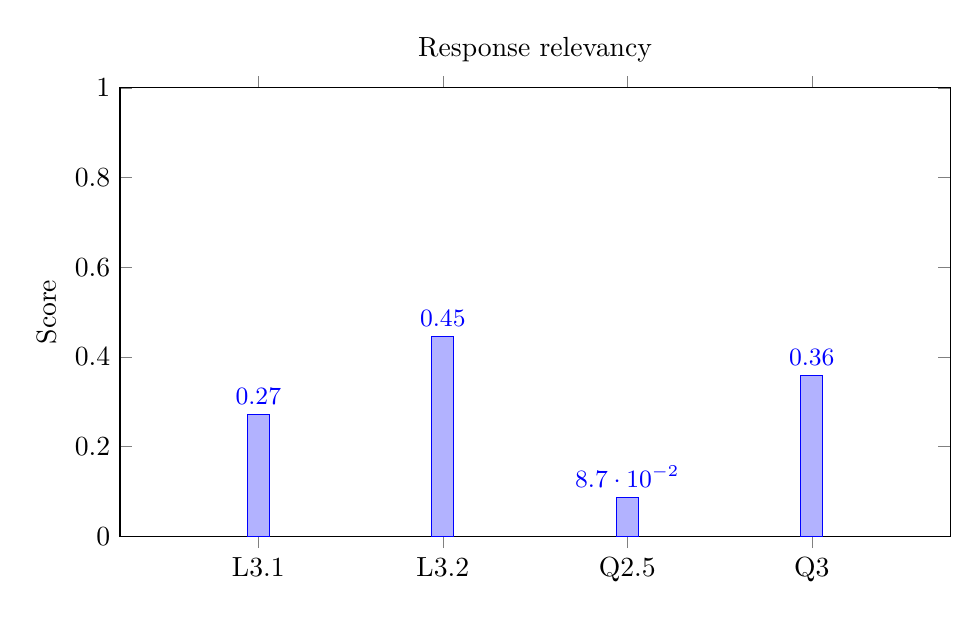
\begin{tikzpicture}
            \begin{axis}[
                ybar,
                ymin=0,
                ymax=1,
                bar width=8pt,
                width=\textwidth,
                height=0.6\textwidth,
                enlarge x limits=0.25,
                ylabel={Score},
                symbolic x coords={L3.1,L3.2,Q2.5,Q3},
                xtick=data,
                nodes near coords,
                nodes near coords align={vertical},
                every node near coord/.append style={font=\small},
                title={Response relevancy}
                ]
                \addplot coordinates {(L3.1,0.272) (L3.2,0.445) (Q2.5,0.087) (Q3,0.358)};
            \end{axis}
        \end{tikzpicture}
    \end{subfigure}
    
    \vspace{1em}
    
    \begin{subfigure}{0.48\textwidth}
        \centering
        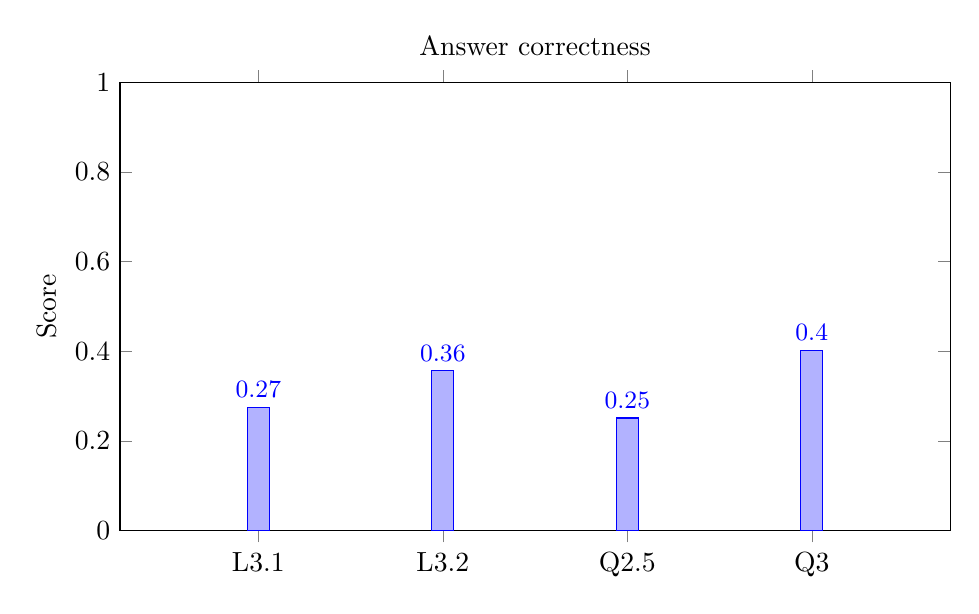
\begin{tikzpicture}
            \begin{axis}[
                ybar,
                ymin=0,
                ymax=1,
                bar width=8pt,
                width=\textwidth,
                height=0.6\textwidth,
                enlarge x limits=0.25,
                ylabel={Score},
                symbolic x coords={L3.1,L3.2,Q2.5,Q3},
                xtick=data,
                nodes near coords,
                nodes near coords align={vertical},
                every node near coord/.append style={font=\small},
                title={Answer correctness}
                ]
                \addplot coordinates {(L3.1,0.274) (L3.2,0.356) (Q2.5,0.251) (Q3,0.402)};
            \end{axis}
        \end{tikzpicture}
    \end{subfigure}
    \hfill
    \begin{subfigure}{0.48\textwidth}
        \centering
        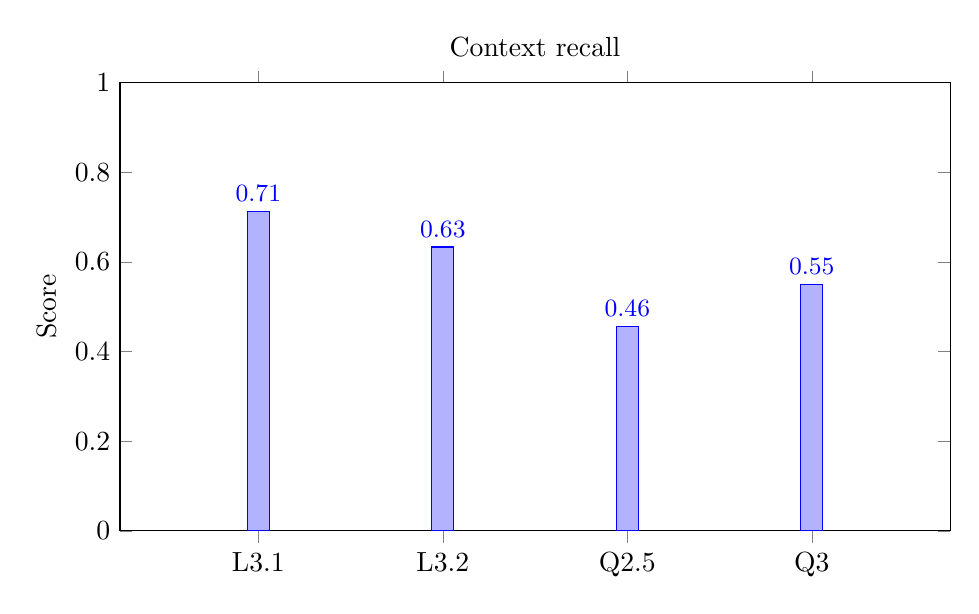
\begin{tikzpicture}
            \begin{axis}[
                ybar,
                ymin=0,
                ymax=1,
                bar width=8pt,
                width=\textwidth,
                height=0.6\textwidth,
                enlarge x limits=0.25,
                ylabel={Score},
                symbolic x coords={L3.1,L3.2,Q2.5,Q3},
                xtick=data,
                nodes near coords,
                nodes near coords align={vertical},
                every node near coord/.append style={font=\small},
                title={Context recall}
                ]
                \addplot coordinates {(L3.1,0.713) (L3.2,0.633) (Q2.5,0.456) (Q3, 0.550)};
            \end{axis}
        \end{tikzpicture}
    \end{subfigure}
    
    \caption{Vergelijking van de prestaties per metric voor alle modellen.}
    \label{fig:vergelijking_metrics}
\end{figure}

Gemiddeld over de vier categorieën scoren de modellen als volgt:

\begin{figure}[H]
    \centering
    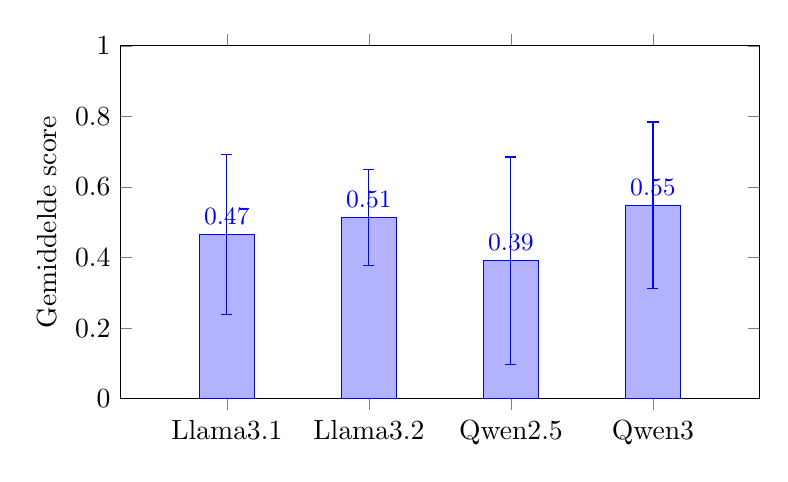
\begin{tikzpicture}
        \begin{axis}[
            ybar,
            ymin=0,
            ymax=1,
            bar width=20pt,
            width=0.8\textwidth,
            height=0.5\textwidth,
            enlarge x limits=0.25,
            ylabel={Gemiddelde score},
            symbolic x coords={Llama3.1,Llama3.2,Qwen2.5,Qwen3},
            xtick=data,
            nodes near coords,
            nodes near coords align={vertical},
            every node near coord/.append style={font=\small}
            ]
            \addplot+[
            error bars/.cd,
            y dir=both,
            y explicit
            ] coordinates {
                (Llama3.1,0.466) +- (0,0.227)
                (Llama3.2,0.514) +- (0,0.136)
                (Qwen2.5,0.391) +- (0,0.294)
                (Qwen3,0.548)   +- (0,0.236)
            };
        \end{axis}
    \end{tikzpicture}
    \caption{Gemiddelde score per model met standaarddeviatie.}
    \label{fig:gemiddelde_score_per_model_met_sd}
\end{figure}


\begin{table}[H]
    \begin{tabular}{|l|c|c|c|c|c|}
        \hline
        \textbf{Model} & \textbf{Faithfulness} & \textbf{Response relevancy} & \textbf{Answer correctness} & \textbf{Context recall} \\
        \hline
        \textbf{llama3.1} & 0.604 & 0.272 & 0.274 & \textbf{0.713} \\
        \textbf{llama3.2} & 0.620 & \textbf{0.445} & 0.356 & 0.633 \\
        \textbf{qwen2.5}  & 0.769 & 0.087 & 0.251 & 0.456 \\
        \textbf{qwen3}    & \textbf{0.880} & 0.358 & \textbf{0.402} & 0.550 \\
        \hline
    \end{tabular}
    \caption{Vergelijking van modelprestaties.}
    \label{tab:modelvergelijking}
\end{table}

\subsection{Bespreking van de resultaten}

%ResponseRelevancy  Scores the relevancy of the answer according to the given question. Answers with incomplete, redundant or unnecessary information is penalized. Score can range from 0 to 1 with 1 being the best.

%Faithfulness The Faithfulness metric measures how factually consistent a response is with the retrieved context. It ranges from 0 to 1, with higher scores indicating better consistency.

% AnswerCorrectness  Measures answer correctness compared to ground truth as a combination of factuality and semantic similarity.

%LLMContextRecall checkt in hoeverre de juiste info voor het antwoord ook effectief aanwezig was in de opgehaalde context. Hoe meer overlap tussen juiste antwoord en context, hoe hoger de score.  aka hoe goed het model zijn retrievalproces heeft aangestuurd.


Uit tabel \ref{tab:modelvergelijking} blijkt dat het model Qwen3 de hoogste scores behaalde voor faithfulness (0.880) en answer correctness (0.402), terwijl Llama3.2 het beste presteerde op response relevancy (0.445) en Llama3.1 op context recall (0.713). 
\\[1em]
Opvallend is dat niet één model op alle gemeten criteria het beste scoorde. Zo behaalde het Qwen3 model de hoogste score op zowel \textit{Faithfulness} als \textit{Answer Correctness}. Dit suggereert dat dit model zich het meest consistent hield aan de geleverde context, en over de hele set van tien vragen ook de meest accurate antwoorden genereerde.
\\[1em]
Voor \textit{Response Relevancy} was het Llama3.2 model de best presterende. De laagste score op deze metric werd echter behaald door het Qwen2.5 model, met een opvallend lage waarde van 0.087. Dit wijst erop dat de antwoorden van dit model vaak irrelevante of overbodige informatie bevatten, of dat cruciale elementen uit het antwoord ontbraken.
\\[1em]
Op het vlak van \textit{Context Recall} scoorde het Llama3.1 model het hoogst, op korte afstand gevolgd door Llama3.2. Dit betekent dat Llama3.1 er het best in slaagde om relevante documentatie op te halen. Toch bleek dit niet automatisch te leiden tot een hoge \textit{Answer Correctness}. Ondanks de hoge context recall, presteerde Llama3.1 relatief zwak op het vlak van antwoordjuistheid. In tegenstelling daarmee behaalde het Qwen3 model wel een hoge answer correctness met een iets lagere context recall, wat impliceert dat het model de opgehaalde informatie beter wist te verwerken en toepassen.
\\[1em]
Gemiddeld scoorde Qwen3 het best, met Llama3.2 op de tweede plaats. Opvallend is dat Llama3.2 slechts drie miljard parameters heeft, tegenover zeven à acht miljard bij de andere modellen, maar toch goed presteerde.
\\[1em]
Figuur \ref{fig:gemiddelde_score_per_model_met_sd} toont bovendien dat Llama3.2 de meest consistente prestaties leverde over de verschillende categorieën, wat bevestigd wordt door de lage standaarddeviatie in vergelijking met de andere modellen. Het model combineert dus een degelijke gemiddelde score met hoge consistentie.

\section{Evaluatie 2: Hallucinaties}

Bij deze test krijgt ieder model een set van 5 vragen voorgeschoteld. Geen van deze vragen komt voor in de documentatie (zie bijlage \ref{hallucinatie-resultaten}) Dit heeft als doel om na te gaan welke modellen tekenen vertonen van hallucinaties en welke niet. 
\\[1em]
De vragenlijst is als volgt:

\begin{enumerate}
    \item Voor welke dienst is Jan Cabooter verantwoordelijk?
    \item Wat is de maximale bestandsgrootte (in MB) die via de repush voor RV kan worden verstuurd?
    \item Wat is de kost voor een Nationality change?
    \item Wat is de technical resource voor DQSS?
    \item Wat is het maximum aantal documenten die kunnen geraadpleegd worden bij myminfin
\end{enumerate}

\begin{table}[H]
    \begin{tabular}{|l|c|c|c|c|}
        \hline
        \textbf{Vraag} & \textbf{Llama3.1} & \textbf{Llama3.2} & \textbf{Qwen2.5} & \textbf{Qwen3} \\
        \hline
       Vraag 1 & Nee & Ja & Nee & Nee \\
       Vraag 2 & Nee & Ja & Ja & Ja \\
       Vraag 3 & Ja & Nee & Nee & Nee \\
       Vraag 4 & Nee & Ja & Nee & Nee \\
       Vraag 5 & Nee & Ja & Nee & Nee \\
        \hline
    \end{tabular}
    \caption{Resultaten hallucinatie test per model bij vragen die niet in de documentatie voorkomen (Ja = hallucinatie, Nee = geen hallucinatie)}
\end{table}

\noindent\textbf{Samenvatting:}  
\begin{table}[H]
    \begin{tabular}{|l|c|}
        \hline
        \textbf{Model} & \textbf{Hallucinatie (\%)} \\
        \hline
        Llama3.1 & 1/5 (20\%) \\
        Llama3.2 & 4/5 (80\%) \\
        Qwen2.5  & 1/5 (20\%) \\
        Qwen3    & 1/5 (20\%) \\
        \hline
    \end{tabular}
    \caption{Samenvatting hallucinatie test}
\end{table}

Uit de resultaten blijkt dat Llama3.2 in 80\% van de gevallen hallucinaties vertoonde, terwijl de overige modellen dit slechts in 20\% van de gevallen deden.

\subsection{Bespreking van de resultaten}

De modellen Qwen3, Qwen2.5 en Llama3.1 vertoonden geen tekenen van hallucinaties. Ze hielden zich goed aan de instructie om geen extra informatie te verzinnen en zich uitsluitend te baseren op de gegevens die in de opgehaalde documenten stonden. Wel ondervond elk van deze modellen problemen bij het beantwoorden van één specifieke vraag. Na nader onderzoek bleek dat, wanneer het model de vraag in het Frans herschreef, de tool call niet altijd correct functioneerde. Het is niet meteen duidelijk waarom dit gebeurde, maar bij de andere vragen traden er bij deze modellen geen hallucinaties op.
\\[1em]
Het Llama3.2-model daarentegen maakte meerdere keren aannames en verzon informatie die niet in de documentatie stond. Dit is uiteraard onwenselijk en kan verstrekkende gevolgen hebben voor de medewerkers die de support verzorgen, wanneer zij deze informatie als juist beschouwen.

\subsubsection{Relevantie voor echte toepassingen}
%Hoe cruciaal is dit type vraag in de praktijk?

Aangezien de opgeleverde informatie wordt gebruikt voor het behandelen van specifieke IT-vragen van burgers over MyMinfin, is het van groot belang dat de modellen geen hallucinaties vertonen. Zelfs wanneer het model uitsluitend informatie levert aan de supportmedewerker, is het essentieel dat deze informatie waarheidsgetrouw is. Op zijn minst moet het model bij twijfel expliciet aangeven dat de benodigde informatie niet beschikbaar is. Op basis van deze test kan het Llama3.2-model niet realistisch worden ingezet.

\section{Evaluatie 3: Triviale vraagstelling}

Tijdens deze test kreeg ieder model een reeks van vijf triviale vragen voorgelegd. De resultaten werden bepaald door de stacktrace van ieder model te analyseren. Op die manier werd vastgesteld of het model de vraag direct beantwoordde of eerst onnodig RAG uitvoerde (zie bijlage \ref{triviale-vragen-resultaten}).
\\[1em]
De vragenlijst is als volgt:

\begin{enumerate}
    \item Hallo hoe gaat het?
    \item Hoeveel dagen zitten er in een week?
    \item Wat is 2 + 2?
    \item In welk land ligt Parijs?
    \item Hoeveel minuten zitten er in een uur?
\end{enumerate}

\begin{table}[H]
    \centering
    \begin{tabular}{|l|c|c|c|c|}
        \hline
        \textbf{Vraag} & \textbf{llama3.1} & \textbf{llama3.2} & \textbf{Qwen2.5} & \textbf{Qwen3} \\
        \hline
        Hallo hoe gaat het? & Nee & Nee & Ja & Ja \\
        Hoeveel dagen zitten er in een week? & Nee & Nee & Ja & Ja \\
        Wat is 2 + 2? & Nee & Nee & Ja & Ja \\
        In welk land ligt Parijs? & Nee & Nee & Ja & Ja \\
        Hoeveel minuten zitten er in een uur? & Nee & Nee & Ja & Ja \\
        \hline
    \end{tabular}
    \caption{Resultaten correct gebruik van de graaf per model bij triviale vragen (verwacht gedrag: direct antwoord, geen RAG)}
\end{table}

\noindent\textbf{Samenvatting:}  
\begin{table}[H]
    \begin{tabular}{|l|c|}
        \hline
        \textbf{Model} & \textbf{Correct (\%)} \\
        \hline
        Llama3.1 & 0/5 (0\%) \\
        Llama3.2 & 0/5 (0\%) \\
        Qwen2.5  & 5/5 (100\%) \\
        Qwen3    & 5/5 (100\%) \\
        \hline
    \end{tabular}
    \caption{Samenvatting van correct gebruik van de graaf per model}
\end{table}

Uit de resultaten blijkt dat Qwen2.5 en Qwen3 alle triviale vragen direct beantwoordden, terwijl Llama3.1 en Llama3.2 in alle gevallen onnodige RAG uitvoerden.

\subsection{Bespreking van de resultaten}
%Verwachtte je een foutloos resultaat?
De resultaten waren in deze vrij duidelijk de 2 Llama modellen slaagde er niet in om een onderscheid te maken tussen triviale en niet-triviale vragen. Dit leidde ertoe dat ze bij iedere vraag het hele ophaal proces gingen gaan uitvoeren. De twee Qwen modellen daarentegen gingen wel meteen antwoorden op de triviale vragen. Met andere woorden is het contrast tussen de Qwen en Llama modellen tijdens deze test vrij groot.
\\[1em]
De resultaten waren in dit geval vrij duidelijk. De twee Llama-modellen slaagden er niet in onderscheid te maken tussen triviale en niet-triviale vragen. Dit leidde ertoe dat zij bij elke vraag het volledige ophaalproces uitvoerden. De twee Qwen-modellen daarentegen gaven direct antwoord op de triviale vragen. Met andere woorden: het contrast tussen de Qwen- en Llama-modellen was tijdens deze test aanzienlijk.

%Werden er toch fouten gemaakt?

\subsubsection{Implicaties resultaten}
%Wat zegt dit over de betrouwbaarheid van het systeem?
Hoewel dit niet direct invloed heeft op de inhoudelijke correctheid van de antwoorden, heeft het wel gevolgen voor de performantie van de toepassing. Bij niet-triviale vragen duurt het beantwoorden aanzienlijk langer bij de Llama-modellen dan bij de Qwen-modellen, omdat bij de Llama-modellen telkens het ophaalproces wordt opgestart.
Voor een consistente en snelle werking van de PoC zijn de Qwen-modellen daardoor beter geschikt dan de Llama-modellen.
%Kunnen deze fouten vermeden worden met betere prompting?


\section{Samenvatting}
%Doel: Alles samenbrengen en overkoepelend reflecteren.
In deze vergelijkende studie werden vier LLM-modellen getest op drie manieren. Namelijk het beantwoorden van vragen op basis van opgehaalde documentatie, het behandelen van vragen die niet in de documentatie voorkwamen en het omgaan met triviale vragen. Elk model werd bij iedere deeltest beoordeeld op zijn prestaties.
\\[1em]
Op basis van deze testen kan worden geconcludeerd dat Qwen3 het beste model is in deze vergelijkende studie. In de eerste test behaalde het model twee keer de hoogste score en één keer de op één na hoogste score. Daarnaast vertoonde het model geen hallucinaties en ging het op een correcte manier om met triviale vragen. Met andere woorden is dit het enige model dat in alle drie de testen aan de verwachtingen voldeed. Op basis van deze resultaten kan worden geconcludeerd dat Qwen3 binnen deze PoC de meest betrouwbare prestaties leverde.